%!TEX TS-program = xelatex
%!TEX encoding = UTF-8 Unicode

\documentclass[12pt]{beamer}
\usepackage{amsmath, fancyvrb, textcomp}
\usepackage{xcolor}
\definecolor{verb}{rgb}{0.0,0.4,0.0}
\definecolor{white}{rgb}{1,1,1}


\let\oldfootnote\footnote
\renewcommand\footnote[1]{\oldfootnote{\scriptsize\ignorespaces#1}}


%% Beamer 版面配置
\beamertemplatenavigationsymbolsempty % 去除 Beamer 導覽工具列
\setbeamertemplate{footline}[frame number]{}
\mode<presentation>
%\usetheme{Frankfurt}
\usecolortheme{whale}
%\usetheme{Madrid}
\useinnertheme{circles}
%\usecolortheme{beaver}
\usefonttheme{structurebold}

%\DefineVerbatimEnvironment{MyVerbatim}{Verbatim}{fontsize=\tiny}

%% 西文字配置
\linespread{1.2}
\usepackage{arevmath}
\usepackage[no-math]{fontspec}
\setmainfont[Mapping=tex-text, LetterSpace=0]{Myriad Pro SemiCondensed}
\setsansfont[Mapping=tex-text, LetterSpace=0]{Myriad Pro SemiCondensed}
%\setmonofont[Color=verb]{Inconsolata}
\setmonofont[Color=verb, Scale=1, LetterSpace=-0]{Consolas}
\usefonttheme{professionalfonts}

%% 中文字配置
\usepackage[
  CJKmath=true, indentfirst=false, PunctStyle={quanjiao}, CheckSingle=false
]{xeCJK}
\setCJKmainfont[Scale=1,BoldFont={AR PChiauHei Extra B5}]{Heiti TC Medium}
\setCJKmonofont[Scale=0.95,BoldFont={AR Yenti Bold B5},Color=verb]{DFYuanBold-B5}

\title[初學者學習R語言]{初學R語言的60分鐘(draft)}
\author[廖鎮磐]{廖鎮磐 \\ \texttt{<andrew.43@gmail.com>}\\ 東海大學生命科學系}
\institute{\normalsize 2015年3月14日於蓮華池}
\date{\footnotesize 
\includegraphics[width=1in]{cc.pdf}\\[5pt]
本文件採用姓名標示-相同方式分享 4.0 國際(CC BY-SA 4.0,詳情請見 \url{http://creativecommons.org/licenses/by-sa/4.0/deed.zh_TW})。}




\AtBeginSection[] {
  \begin{frame}
    \frametitle{大綱}
    \tableofcontents[currentsection]
  \end{frame}
  \addtocounter{framenumber}{-1}
} 

\begin{document}


\begin{frame}
\titlepage
\end{frame}

\begin{frame}{歡迎下載本投影片複本}
\begin{center}

\includegraphics[width=2.75in]{url.pdf}\\
\footnotesize\url{http://www.slideshare.net/chenpanliao/slide-44171070}
\end{center}
\end{frame}

\begin{frame}{我今天希望讓諸位達成\ldots\ldots}
\begin{itemize}
\item 不怕害使用R這類以文字指令進行的工作方式。
\item 自己救自己。
\item 請別人救自己。
\item 實作一些常見的統計分析與繪圖。
\end{itemize}
\end{frame}


\begin{frame}
\frametitle{大綱}
\tableofcontents
\end{frame}

\section{事前準備}\subsection{}


\begin{frame}{為什麼我選擇R?}
\begin{itemize}
\item 自由、免費、跨平台。
\item 是一種「程式語言」,像Python、Perl、JAVA等。
\item 是一種「統計工具」,像SAS、SPSS等。
\item 強大的視覺化工具,畫專業的圖,但需要經驗。
\item 套件豐富,不同自己重新寫程式。
\end{itemize}
%\begin{block}{怎麼入門?}
%\begin{itemize}
%\item 買(可能不只一本)書。
%\item 網路教學和論壇。
%\end{itemize}
%\end{block}
\end{frame}

\begin{frame}[fragile]{安裝R語言}
\begin{enumerate}
\item 到達 \url{http://www.r-project.org/}
\item 點選Download, Packages (CRAN) \\
\item 選擇作業平台
	\begin{center}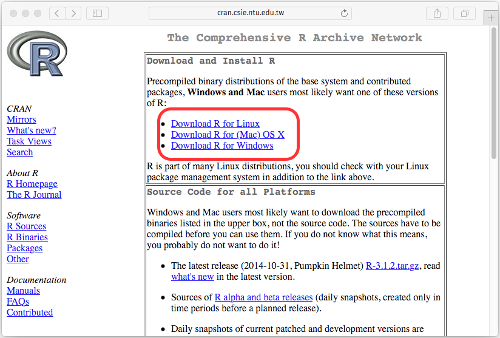
\includegraphics[width=0.7\textwidth]{downloadR.png}\end{center}
\end{enumerate}
\end{frame}

\begin{frame}[fragile]{選用適當的R程式編輯器}
\begin{itemize}
\item 建議以純文字編輯器撰寫R程式碼,並儲存成「\verb+.R+」檔。
\item 「語法多色支援」、「語法提示」、「即時執行」等功能,增加撰寫效率。
\item 支援R語言的編輯器很多,有興趣請自行試用。
\begin{description}
	\item [RStudio] 強大、整合性高、專為R程式員設計。\footnote{\url{http://www.rstudio.com/}}
	\item [Notepad++] 老字號的純文字編輯器,有和R相配合的外掛。\footnote{\url{http://notepad-plus-plus.org/}}
	\item [Atom] 與GitHub配合度高。\footnote{\url{https://atom.io/}}
\end{description}
\end{itemize}
\end{frame}


\begin{frame}[fragile]{R的套件}
\begin{block}{什麼是套件(package)?}
安裝在R系統裡的外掛,讓你「不用重新造輪子」。
\end{block}

\begin{block}{如何安裝、更新及引入套件?}
\begin{itemize}
\item 連上網路之後,輸入
\verb+install.packages("套件名稱")+
可以安裝某套件,而
\verb+update.packages()+
可以更新所有已安裝套件。

\item 在已安裝某套件之後,輸入
\verb+library(套件名稱)+
可引入該套件,之後才可以使用它的功能。
\end{itemize}
\end{block}

\begin{block}{練習}
安裝一個名叫「\verb+vegan+」的套件,並將之引入R中。
\end{block}
\end{frame}

\begin{frame}[fragile]{R的官方套件庫}
\begin{itemize}
\item \url{http://cran.r-project.org/web/packages/available_packages_by_name.html}\\
官方的套件一覽表(目前有6,000多個)。
\item 「我如何找能做某件事的套作?」「有沒有什麼方式可以快速找到我需要哪個套件?」
\item 阿盤:「我都是請谷歌大神幫我找的。」
\end{itemize}
\end{frame}


\section{R的函數}\subsection{}

\begin{frame}[fragile]{什麼是程式語言的函數(function)}
\begin{itemize}
\item 操作R的過程,幾乎就是使用各種function的過程。
\item 就像數學裡的函數一樣:把x放到f裡,得到一個f(x)。
\item x稱為引數,而f(x)叫回傳值。
\item 使用某函數的語法通則: \\ \verb+函數名(第一引數名 = 某值, 第二引數名 = 某值, ...)+ 
\item 試試看 \verb+seq(from = 0, to = 9)+ 的回傳值是什麼?
\item 用中文說明上面的程式:「在 \verb+seq()+ 這個function中,第一個引數名為 \verb+from+,表示起始值,其值為 \verb+0+;第二個引數名為 \verb+to+,表示終點值,其值是 \verb+9+。」
\end{itemize}
\end{frame}



\begin{frame}[fragile]{函數的使用手冊}
\begin{itemize}
\item 觀看某個函數的使用手冊:\verb+?函數名+ 或 \verb+help(函數名)+。
\item 使用手冊中都有以下資訊:
\begin{description}
	\item [Description] 函數的功能。
	\item [Usage] 基本語法,包括了引數的順序和預設值。
	\item [Arguments] 引數的細節。
	\item [Details] 函數的詳細內容。
	\item [Value] 回傳值的內容。
	\item [See Also] 其它相關的函數。
	\item [Examples] 使用範例。
\end{description}
\end{itemize}
\end{frame}



\begin{frame}[fragile]{引數的預設值}

\begin{block}{\texttt{seq()} 的使用語法}
\verb+seq(from = 1, to = 1, ...)+ \\
\end{block}
\begin{itemize}
\item 在使用手冊中可以看出:
  \\ 第一個引數 \verb+from+ 的預設值是 1。
  \\ 第一個引數 \verb+to+ 的預設值是 1。
\item 使用者未定義時採用的值,就是預設值。
\item 方便快速使用。
\item 例如:\\
  \verb+seq(from = 10)+ 和 \\
  \verb+seq(from = 10, to = 1)+ 是相等的。
\end{itemize}
\end{frame}


\begin{frame}[fragile]{引數的順序}

\begin{block}{\texttt{seq()}的使用語法}
\verb+seq(from = 1, to = 1, ...)+ \\
\end{block}

\begin{itemize}
\item 當明確指定引數名時,引數的順序無所謂。例如:\\ \verb+seq(from = 0, to = 9)+ 和 \\ \verb+seq(to = 9, from = 0)+ 同義。
\item 當引數的順序與該函數要求的順序相同時,可以省略引數名。例如:\\ \verb+seq(from = 0, to = 9)+ 可以省略為 \\ \verb+seq(0, 9)+。
\end{itemize}
\end{frame}


\begin{frame}[fragile]{引數的綜合練習}

\begin{block}{\texttt{seq()}的使用語法}
\verb+seq(from = 1, to = 1, ...)+ \\
\end{block}

\begin{block}{試回答下列程式的回傳值為何?}
\begin{itemize}
\item \verb+seq(from = 3, to = 1)+
\item \verb+seq(3, to = 1)+
\item \verb+seq(from = 3, 1)+
\item \verb+seq(3, 1)+
\item \verb+seq(to = 1, from = 3)+
\end{itemize}
\end{block}
\end{frame}

\section{資料的讀取與整理}\subsection{}


\section{小試身手}\subsection{}

\begin{frame}[fragile]{計算機}
\begin{verbatim}
> 2.4 + 42
[1] 44.4
> sqrt(100)
[1] 10
\end{verbatim}
\end{frame}




\end{document}